%============================================================
%  CUSTOMER CARE OPERATIONAL MANUAL
%  Engineer: Abdulrahman Hamdi — AI Engineer
%  Compile: pdflatex x2
%============================================================
\documentclass[11pt,a4paper]{article}

\usepackage[T1]{fontenc}
\usepackage[utf8]{inputenc}
\usepackage{mathptmx}
\usepackage[scaled=0.92]{helvet}
\usepackage{courier}
\usepackage{microtype}
\usepackage[top=2.5cm,bottom=2.5cm,left=2.5cm,right=2.5cm,headheight=16pt]{geometry}
\usepackage{xcolor}
\usepackage{graphicx}
\usepackage{amsmath}
\usepackage{booktabs}
\usepackage{array}
\usepackage{colortbl}
\usepackage{multicol}
\usepackage{enumitem}
\usepackage{fancyhdr}
\usepackage{titlesec}
\usepackage{tcolorbox}
\usepackage{tikz}
\usepackage{mdframed}
\usepackage{hyperref}
\usepackage{tabularx}

\usetikzlibrary{shapes.geometric,arrows.meta,positioning,fit,calc,shadows,backgrounds}
\tcbuselibrary{skins,breakable}

%-----------------------------------------------------------
% COLOURS
%-----------------------------------------------------------
\definecolor{PrimaryBlue}{HTML}{1A3C5E}
\definecolor{AccentTeal}{HTML}{0D7C8C}
\definecolor{AccentGold}{HTML}{C8962A}
\definecolor{LightBg}{HTML}{F4F7FA}
\definecolor{MidGray}{HTML}{6B7B8D}
\definecolor{DangerRed}{HTML}{C0392B}
\definecolor{SuccessGreen}{HTML}{1E8449}
\definecolor{WarningAmber}{HTML}{D4850A}
\definecolor{SoftBlue}{HTML}{D6E4F0}
\definecolor{SoftTeal}{HTML}{D0EEF2}
\definecolor{SoftGold}{HTML}{FAF0DC}
\definecolor{SoftRed}{HTML}{FADBD8}
\definecolor{SoftGreen}{HTML}{D5F5E3}
\definecolor{TableHead}{HTML}{1A3C5E}
\definecolor{TableAlt}{HTML}{EAF2FA}
\definecolor{RuleColor}{HTML}{B0C4D8}

%-----------------------------------------------------------
% HYPERREF
%-----------------------------------------------------------
\hypersetup{colorlinks=true,linkcolor=PrimaryBlue,urlcolor=AccentTeal,
  pdftitle={Operational Manual: Customer Care --- AI Dept.},bookmarksnumbered=true}

%-----------------------------------------------------------
% HEADER / FOOTER
%-----------------------------------------------------------
\pagestyle{fancy}\fancyhf{}
\fancyhead[L]{\color{MidGray}\small\textit{Customer Care \& Patient Journey --- AI Department}}
\fancyhead[R]{\color{MidGray}\small\textit{Eng.\ Abdulrahman Hamdi}}
\fancyfoot[C]{\color{MidGray}\thepage}
\renewcommand{\headrulewidth}{0.4pt}
\renewcommand{\headrule}{\hbox to\headwidth{\color{RuleColor}\leaders\hrule height\headrulewidth\hfill}}

%-----------------------------------------------------------
% SECTION STYLING
%-----------------------------------------------------------
\titleformat{\section}{\color{PrimaryBlue}\Large\bfseries}
  {\colorbox{PrimaryBlue}{\color{white}\ \thesection\ }}{0.8em}{}
  [\vspace{-0.2em}\color{RuleColor}\rule{\linewidth}{1.5pt}\vspace{0.3em}]
\titleformat{\subsection}{\color{AccentTeal}\large\bfseries}
  {\color{AccentTeal}\thesubsection}{0.6em}{}
  [\vspace{-0.3em}\color{RuleColor}\rule{\linewidth}{0.6pt}]
\titleformat{\subsubsection}{\color{PrimaryBlue}\normalsize\bfseries}
  {\color{AccentGold}\thesubsubsection}{0.5em}{}
\titlespacing*{\section}{0pt}{1.6em}{0.8em}
\titlespacing*{\subsection}{0pt}{1.2em}{0.5em}
\titlespacing*{\subsubsection}{0pt}{0.9em}{0.3em}

%-----------------------------------------------------------
% LISTS
%-----------------------------------------------------------
\setlist[itemize,1]{label={\color{AccentTeal}\textbullet},leftmargin=1.5em,itemsep=0.25em,topsep=0.3em}
\setlist[itemize,2]{label={\color{AccentGold}\small$\blacktriangleright$},leftmargin=1.5em,itemsep=0.15em}
\setlist[enumerate,1]{label={\color{PrimaryBlue}\bfseries\arabic*.},leftmargin=1.8em,itemsep=0.25em}

%-----------------------------------------------------------
% TCOLORBOX STYLES
%-----------------------------------------------------------
\tcbset{
  infobox/.style={enhanced,breakable,colback=SoftBlue,colframe=PrimaryBlue,
    boxrule=1.2pt,arc=4pt,left=8pt,right=8pt,top=6pt,bottom=6pt,
    fonttitle=\bfseries\color{white},
    attach boxed title to top left={yshift=-2mm,xshift=6mm},
    boxed title style={colback=PrimaryBlue,arc=3pt,boxrule=0pt}},
  warnbox/.style={enhanced,breakable,colback=SoftGold,colframe=WarningAmber,
    boxrule=1.2pt,arc=4pt,left=8pt,right=8pt,top=6pt,bottom=6pt,
    fonttitle=\bfseries\color{white},
    attach boxed title to top left={yshift=-2mm,xshift=6mm},
    boxed title style={colback=WarningAmber,arc=3pt,boxrule=0pt}},
  dangerbox/.style={enhanced,breakable,colback=SoftRed,colframe=DangerRed,
    boxrule=1.2pt,arc=4pt,left=8pt,right=8pt,top=6pt,bottom=6pt,
    fonttitle=\bfseries\color{white},
    attach boxed title to top left={yshift=-2mm,xshift=6mm},
    boxed title style={colback=DangerRed,arc=3pt,boxrule=0pt}},
  successbox/.style={enhanced,breakable,colback=SoftGreen,colframe=SuccessGreen,
    boxrule=1.2pt,arc=4pt,left=8pt,right=8pt,top=6pt,bottom=6pt,
    fonttitle=\bfseries\color{white},
    attach boxed title to top left={yshift=-2mm,xshift=6mm},
    boxed title style={colback=SuccessGreen,arc=3pt,boxrule=0pt}},
  statbox/.style={enhanced,colback=LightBg,colframe=AccentGold,
    boxrule=2pt,arc=6pt,left=10pt,right=10pt,top=8pt,bottom=8pt},
  rulebox/.style={enhanced,breakable,colback=LightBg,colframe=PrimaryBlue,
    boxrule=0.8pt,arc=3pt,left=7pt,right=7pt,top=6pt,bottom=6pt,
    borderline west={3pt}{0pt}{AccentTeal}},
  metricbox/.style={enhanced,colback=white,colframe=AccentTeal,
    boxrule=1.4pt,arc=6pt,left=8pt,right=8pt,top=8pt,bottom=8pt,
    drop shadow}
}

%-----------------------------------------------------------
% TIKZ BASE STYLES
% NB: ALL nodes use align=center so \\ works inside node text
%-----------------------------------------------------------
\tikzset{
  % Base box
  FB/.style={rectangle,rounded corners=3pt,
             minimum width=2.6cm,minimum height=0.85cm,
             text centered,align=center,draw,thick,
             font=\footnotesize\bfseries},
  % Base diamond
  DM/.style={diamond,aspect=2.0,
             minimum width=2.4cm,minimum height=0.75cm,
             text centered,align=center,draw,thick,
             font=\footnotesize\bfseries},
  % Arrow
  arr/.style={-{Stealth[length=4.5pt]},thick},
  % Colour variants
  nB/.style={FB,fill=SoftBlue, draw=PrimaryBlue,text=PrimaryBlue},
  nT/.style={FB,fill=SoftTeal, draw=AccentTeal, text=AccentTeal},
  nG/.style={FB,fill=SoftGold, draw=AccentGold, text=AccentGold},
  nR/.style={FB,fill=SoftRed,  draw=DangerRed,  text=DangerRed},
  nV/.style={FB,fill=SoftGreen,draw=SuccessGreen,text=SuccessGreen},
  dB/.style={DM,fill=SoftBlue, draw=PrimaryBlue,text=PrimaryBlue},
  dT/.style={DM,fill=SoftTeal, draw=AccentTeal, text=AccentTeal},
  % Label styles
  LY/.style={font=\scriptsize\bfseries\color{SuccessGreen},midway,auto},
  LN/.style={font=\scriptsize\bfseries\color{DangerRed},midway,auto}
}

%-----------------------------------------------------------
% HELPERS
%-----------------------------------------------------------
\newcolumntype{L}[1]{>{\raggedright\arraybackslash}p{#1}}
\newcolumntype{C}[1]{>{\centering\arraybackslash}p{#1}}

%============================================================
\begin{document}
%============================================================

%------------------------------------------------------------
% COVER PAGE
%------------------------------------------------------------
\begin{titlepage}
\pagecolor{PrimaryBlue}\color{white}
\vspace*{1.0cm}
\begin{center}
  \textcolor{AccentGold}{\rule{0.88\linewidth}{2pt}}\\[0.3em]
  \textcolor{AccentGold}{\rule{0.88\linewidth}{0.5pt}}\\[2.0cm]

  {\fontsize{38}{46}\selectfont\bfseries Comprehensive}\\[0.2em]
  {\fontsize{28}{36}\selectfont\bfseries Operational Manual}\\[1.0em]

  \textcolor{AccentGold}{\rule{0.5\linewidth}{0.8pt}}\\[0.8em]
  {\Large Customer Care \& Patient Journey}\\[0.4em]
  {\color{SoftBlue}\small
    Patient Acquisition \textbullet{} Retention \textbullet{}
    Schedule Optimization \textbullet{} Cash Flow Preservation}\\[2.8cm]

  \begin{tabular}{@{}ll@{}}
    \textcolor{AccentGold}{\bfseries Department:} & Customer Care \\[0.3em]
    \textcolor{AccentGold}{\bfseries Prepared by:} & Eng.\ Abdulrahman Hamdi --- AI Engineer \\[0.3em]
    \textcolor{AccentGold}{\bfseries Version:} & 1.0 \\[0.3em]
    \textcolor{AccentGold}{\bfseries Year:} & 2026 \\
  \end{tabular}

  \vfill
  \textcolor{AccentGold}{\rule{0.88\linewidth}{0.5pt}}\\[0.3em]
  \textcolor{AccentGold}{\rule{0.88\linewidth}{2pt}}
\end{center}
\end{titlepage}
\nopagecolor\color{black}

%------------------------------------------------------------
% TABLE OF CONTENTS
%------------------------------------------------------------
\newpage
\tableofcontents
\newpage

%============================================================
\section*{Executive Operating Snapshot}
\addcontentsline{toc}{section}{Executive Operating Snapshot}
%============================================================

\begin{tcolorbox}[statbox]
\begin{center}
  \Large\bfseries\color{PrimaryBlue}Management Objective\\[0.4em]
  \normalsize
  Map the complete Customer Care operating model from first patient contact through
  scheduling, insurance control, attendance management, discharge, and billing readiness.
  Every rule in this manual protects one of four outcomes:
\end{center}

\vspace{0.3em}
\begin{center}
\begin{tabularx}{0.96\linewidth}{C{3.1cm} C{3.1cm} C{3.1cm} C{3.1cm}}
  \textcolor{PrimaryBlue}{\bfseries Acquisition} &
  \textcolor{AccentTeal}{\bfseries Retention} &
  \textcolor{AccentGold}{\bfseries Capacity} &
  \textcolor{DangerRed}{\bfseries Cash Flow} \\
  New lead capture &
  Future visits booked &
  Green Board protected &
  Denials prevented \\
\end{tabularx}
\end{center}
\end{tcolorbox}

\begin{tcolorbox}[rulebox,title={Operating Principle}]
Customer Care is not only a communication function. It is a revenue-control function.
An incorrect case selection, expired authorization, missed hold status, or incomplete
check-out can convert a treated visit into an unbillable visit.
\end{tcolorbox}


%============================================================
\section{Software \& Tool Ecosystem}
%============================================================

The department operates through a tightly integrated suite of platforms.
Each tool serves a specific role in the patient lifecycle pipeline.

\vspace{0.5em}
% 2x3 grid — each row fits inside text width safely
\begin{center}
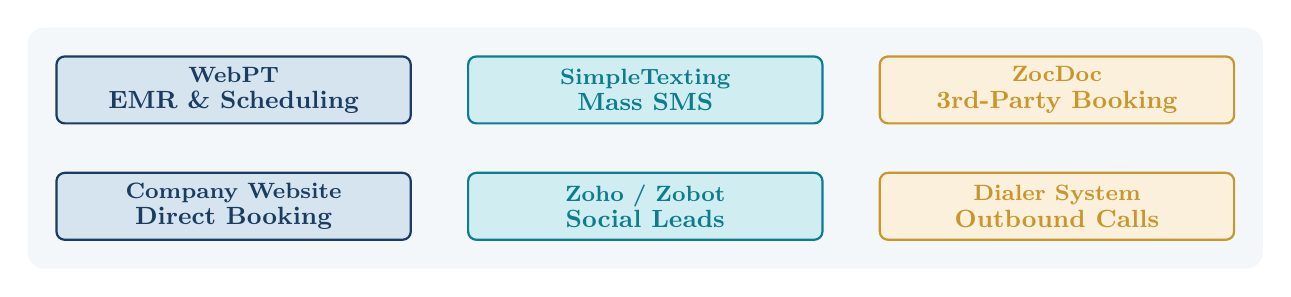
\begin{tikzpicture}[node distance=0.5cm and 0.8cm]
  \node[nB,minimum width=4.5cm] (webpt)  {WebPT \\ \small EMR \& Scheduling};
  \node[nT,minimum width=4.5cm,right=0.7cm of webpt]  (simple) {SimpleTexting \\ \small Mass SMS};
  \node[nG,minimum width=4.5cm,right=0.7cm of simple] (zocdoc) {ZocDoc \\ \small 3rd-Party Booking};
  \node[nB,minimum width=4.5cm,below=0.6cm of webpt]  (web)    {Company Website \\ \small Direct Booking};
  \node[nT,minimum width=4.5cm,right=0.7cm of web]    (zoho)   {Zoho / Zobot \\ \small Social Leads};
  \node[nG,minimum width=4.5cm,right=0.7cm of zoho]   (dialer) {Dialer System \\ \small Outbound Calls};
  \begin{scope}[on background layer]
    \node[fill=LightBg,rounded corners=6pt,inner sep=10pt,
          fit=(webpt)(simple)(zocdoc)(web)(zoho)(dialer)] {};
  \end{scope}
\end{tikzpicture}
\end{center}
\vspace{0.5em}

\begin{tcolorbox}[infobox,title={Tool Reference Table}]
\begin{tabularx}{\linewidth}{L{2.6cm} X L{3.0cm}}
  \rowcolor{TableHead}
  \color{white}\textbf{Tool} & \color{white}\textbf{Function} & \color{white}\textbf{Primary User} \\
  \textbf{WebPT}        & EMR: chart creation, Green Board scheduling, clinical documentation & All teams \\
  \rowcolor{TableAlt}
  \textbf{SimpleTexting}& Mass SMS confirmations (C\,/\,R\,/\,X campaigns) & Back Office \\
  \textbf{ZocDoc}       & Third-party self-booking portal (similar to Vezeeta) & Patients / Offline Desk \\
  \rowcolor{TableAlt}
  \textbf{Website}      & Direct booking with demographics \& insurance upload & Patients / Offline Desk \\
  \textbf{Zoho (Zobot)} & Lead management from social media (Instagram, Twitter, LinkedIn) & Offline Desk \\
  \rowcolor{TableAlt}
  \textbf{Dialer}       & Outbound call management \& disposition tracking & Back Office / Front Line \\
\end{tabularx}
\end{tcolorbox}

%============================================================
\section{Departmental Structure \& Pillars}
%============================================================

The Customer Care department is divided into \textbf{four operational lines of business}.

\vspace{0.4em}
\begin{center}
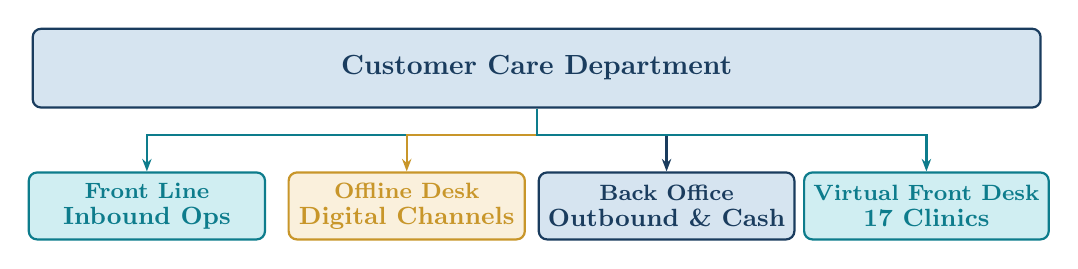
\begin{tikzpicture}[x=1cm,y=1cm]
  % Fixed-width layout kept safely inside the text block.
  \node[nB,minimum width=12.8cm,minimum height=1cm,font=\bfseries\normalsize] (dept) at (0,0)
    {Customer Care Department};
  \coordinate (hub) at (0,-0.85);
  \node[nT,minimum width=3.0cm] (fl)  at (-4.95,-1.75)
    {Front Line \\ \small Inbound Ops};
  \node[nG,minimum width=3.0cm] (od)  at (-1.65,-1.75)
    {Offline Desk \\ \small Digital Channels};
  \node[nB,minimum width=3.0cm] (bo)  at (1.65,-1.75)
    {Back Office \\ \small Outbound \& Cash};
  \node[nT,minimum width=3.0cm] (vfd) at (4.95,-1.75)
    {Virtual Front Desk \\ \small 17 Clinics};
  \draw[arr,AccentTeal]  (dept.south) -- (hub) -| (fl.north);
  \draw[arr,AccentGold]  (dept.south) -- (hub) -| (od.north);
  \draw[arr,PrimaryBlue] (dept.south) -- (hub) -| (bo.north);
  \draw[arr,AccentTeal]  (dept.south) -- (hub) -| (vfd.north);
\end{tikzpicture}
\end{center}

%------------------------------------------------------------
\subsection{Front Line --- Inbound Operations}
%------------------------------------------------------------

The Front Line team receives all inbound calls and is responsible for new patient onboarding following a strict sequential order.

\begin{tcolorbox}[successbox,title={Front Line SOP --- Sequential Steps}]
\begin{enumerate}
  \item \textbf{Patient Intake:} Collect full demographic, contact, referral, and insurance information.
  \item \textbf{Chart Creation:} Generate a new chart in WebPT \emph{before} any scheduling action.
  \item \textbf{Case Accuracy Check:} If the patient is returning, confirm whether the visit belongs to an existing active case or a new case.
  \item \textbf{Pre-Scheduling:} Secure the requested time slot \emph{before} eligibility is finalized to protect the lead.
  \item \textbf{Eligibility Check:} Coordinate with the Benefits Team to verify active coverage, authorization rules, and visit limits.
  \item \textbf{Patient Notification:} Confirm eligible appointments; cancel and notify ineligible patients before treatment occurs.
\end{enumerate}
\end{tcolorbox}

\begin{tcolorbox}[dangerbox,title={Front Line Billing Control Point}]
The highest-risk intake mistake is scheduling a returning patient under the wrong WebPT case.
If the patient is being treated for a new body part, the appointment must not be attached to a closed or unrelated case.
\end{tcolorbox}

\vspace{0.4em}
% Vertical flowchart — safe for any page width
\begin{center}
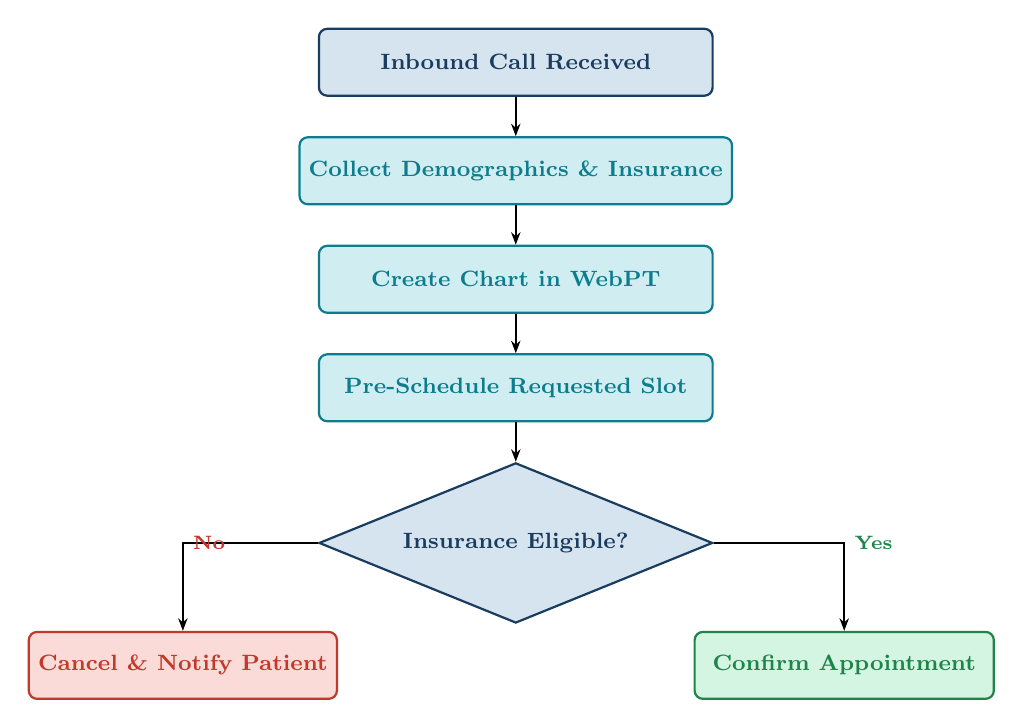
\begin{tikzpicture}[node distance=0.55cm,every node/.style={align=center}]
  \node[nB,minimum width=5cm]                 (call)    {Inbound Call Received};
  \node[nT,minimum width=5cm,below=0.5cm of call]  (intake)  {Collect Demographics \& Insurance};
  \node[nT,minimum width=5cm,below=0.5cm of intake](chart)   {Create Chart in WebPT};
  \node[nT,minimum width=5cm,below=0.5cm of chart] (presched){Pre-Schedule Requested Slot};
  \node[dB,minimum width=5cm,below=0.5cm of presched](elig)  {Insurance Eligible?};
  \node[nV,minimum width=3.8cm,below right=0.6cm and 1.0cm of elig] (yes){Confirm Appointment};
  \node[nR,minimum width=3.8cm,below left=0.6cm  and 1.0cm of elig] (no) {Cancel \& Notify Patient};

  \draw[arr](call)--(intake);
  \draw[arr](intake)--(chart);
  \draw[arr](chart)--(presched);
  \draw[arr](presched)--(elig);
  \draw[arr](elig.east)  -| node[LY]{Yes} (yes.north);
  \draw[arr](elig.west)  -| node[LN]{No}  (no.north);
\end{tikzpicture}
\end{center}

%------------------------------------------------------------
\subsection{Offline Desk --- Digital Channel Operations}
%------------------------------------------------------------

This team manages all asynchronous digital bookings from ZocDoc, the website, and social media.

\begin{tcolorbox}[infobox,title={Offline Desk Key Rules}]
\begin{itemize}
  \item \textbf{Source Coverage:} ZocDoc, company website, and Zoho/Zobot social leads are all treated as active booking queues.
  \item \textbf{Queue Management:} Every requested time is cross-referenced against WebPT availability and Green Board capacity.
  \item \textbf{Conflict Resolution:} If time unavailable --- call first, then SMS if no answer.
  \item \textbf{Force Scheduling Exception:} If patient remains unresponsive, override only as a lead-preservation exception and flag for follow-up.
  \item \textbf{Hard Deadline:} Queue \emph{must} be closed by \textbf{3:00 PM} daily.
\end{itemize}
\end{tcolorbox}

\begin{tcolorbox}[warnbox,title={Offline Desk 3:00 PM Closure Rule}]
The 3:00 PM deadline is an operational control, not an administrative preference.
If the digital queue remains open after 3:00 PM, next-day schedules may show inaccurate capacity,
unconfirmed arrivals, or unresolved conflicts.
\end{tcolorbox}

\vspace{0.4em}
\begin{center}
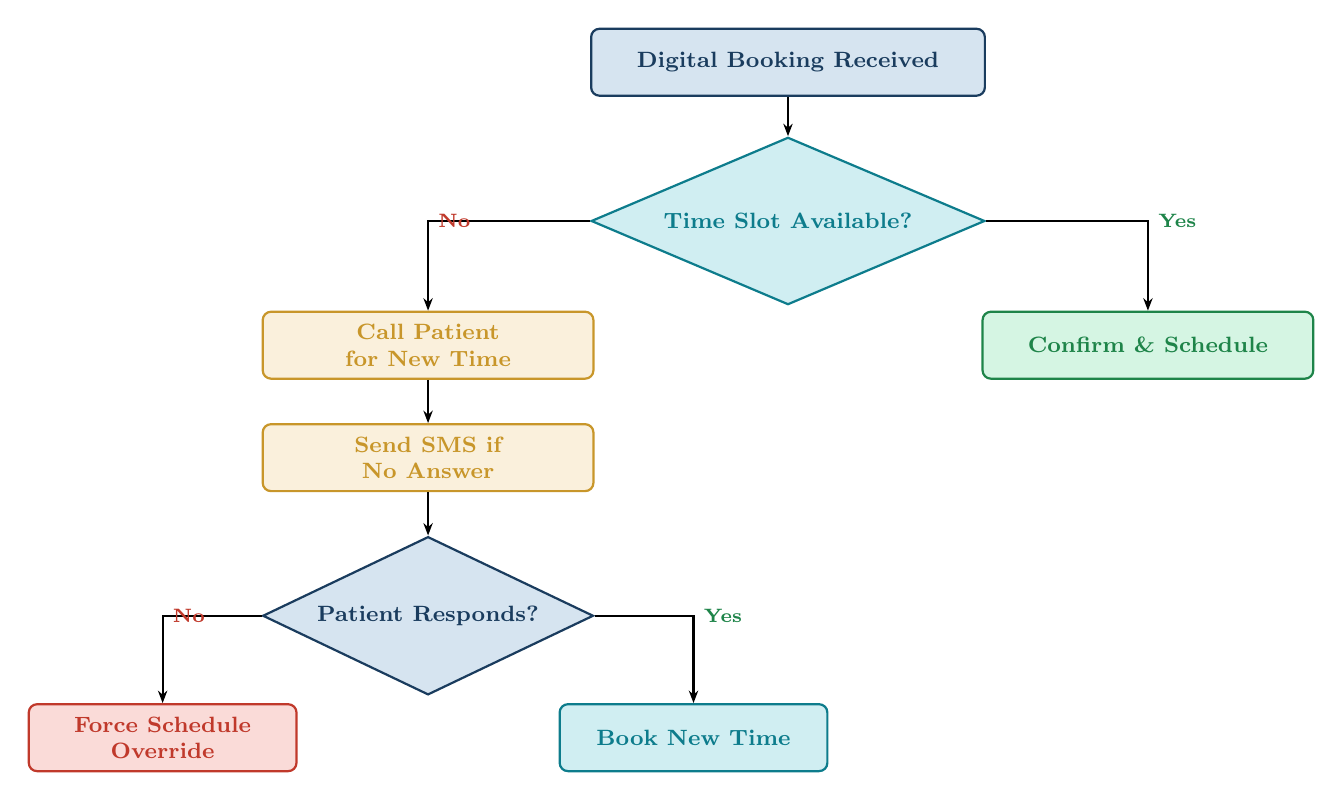
\begin{tikzpicture}[node distance=0.55cm,every node/.style={align=center}]
  \node[nB,minimum width=5cm]                  (book) {Digital Booking Received};
  \node[dT,minimum width=5cm,below=0.5cm of book]     (avail){Time Slot Available?};
  \node[nV,minimum width=4.2cm,below right=0.6cm and 1.2cm of avail] (conf) {Confirm \& Schedule};
  \node[nG,minimum width=4.2cm,below left=0.6cm  and 1.2cm of avail] (callp){Call Patient \\ for New Time};
  \node[nG,minimum width=4.2cm,below=0.55cm of callp]  (sms)  {Send SMS if \\ No Answer};
  \node[dB,minimum width=4.2cm,below=0.55cm of sms]    (ans)  {Patient Responds?};
  \node[nT,minimum width=3.4cm,below right=0.6cm and 0.6cm of ans] (rebook){Book New Time};
  \node[nR,minimum width=3.4cm,below left=0.6cm  and 0.6cm of ans] (force) {Force Schedule \\ Override};

  \draw[arr](book)--(avail);
  \draw[arr](avail.east)  -| node[LY]{Yes} (conf.north);
  \draw[arr](avail.west)  -| node[LN]{No}  (callp.north);
  \draw[arr](callp)--(sms);
  \draw[arr](sms)--(ans);
  \draw[arr](ans.east) -| node[LY]{Yes} (rebook.north);
  \draw[arr](ans.west) -| node[LN]{No}  (force.north);
\end{tikzpicture}
\end{center}

%------------------------------------------------------------
\subsection{Green Board Scheduling Rules}
%------------------------------------------------------------

Scheduling is governed by the \textbf{Green Board} --- strict clinical capacity guidelines dictating how many patients a PT can see per time block.

\begin{tcolorbox}[warnbox,title={Green Board Capacity Rules}]
\begin{tabularx}{\linewidth}{L{3.8cm} X}
  \rowcolor{TableHead}
  \color{white}\textbf{Visit Type} & \color{white}\textbf{Rule} \\
  \textbf{Follow-up}       & 1 slot (30-minute unit) \\
  \rowcolor{TableAlt}
  \textbf{Initial Exam}    & 2 slots (equals 2 follow-ups) \\
  \textbf{Re-examination}  & Special type --- highlighted \textcolor{DangerRed}{\textbf{red}} in WebPT \\[0.3em]
  \rowcolor{TableHead}
  \color{white}\textbf{Restriction} & \color{white}\textbf{Rule} \\
  \textbf{Back-to-back Initials} & \textcolor{DangerRed}{\bfseries PROHIBITED} --- must have 1-hour gap \\
  \rowcolor{TableAlt}
  \textbf{Simultaneous Initials} & Allowed only if total capacity permits \\
  \textbf{Capacity Breach} & 3 follow-ups + 1 Initial = 5 slots $\rightarrow$ \textcolor{DangerRed}{\bfseries VIOLATION} \\
\end{tabularx}
\end{tcolorbox}

\vspace{0.4em}
\begin{center}
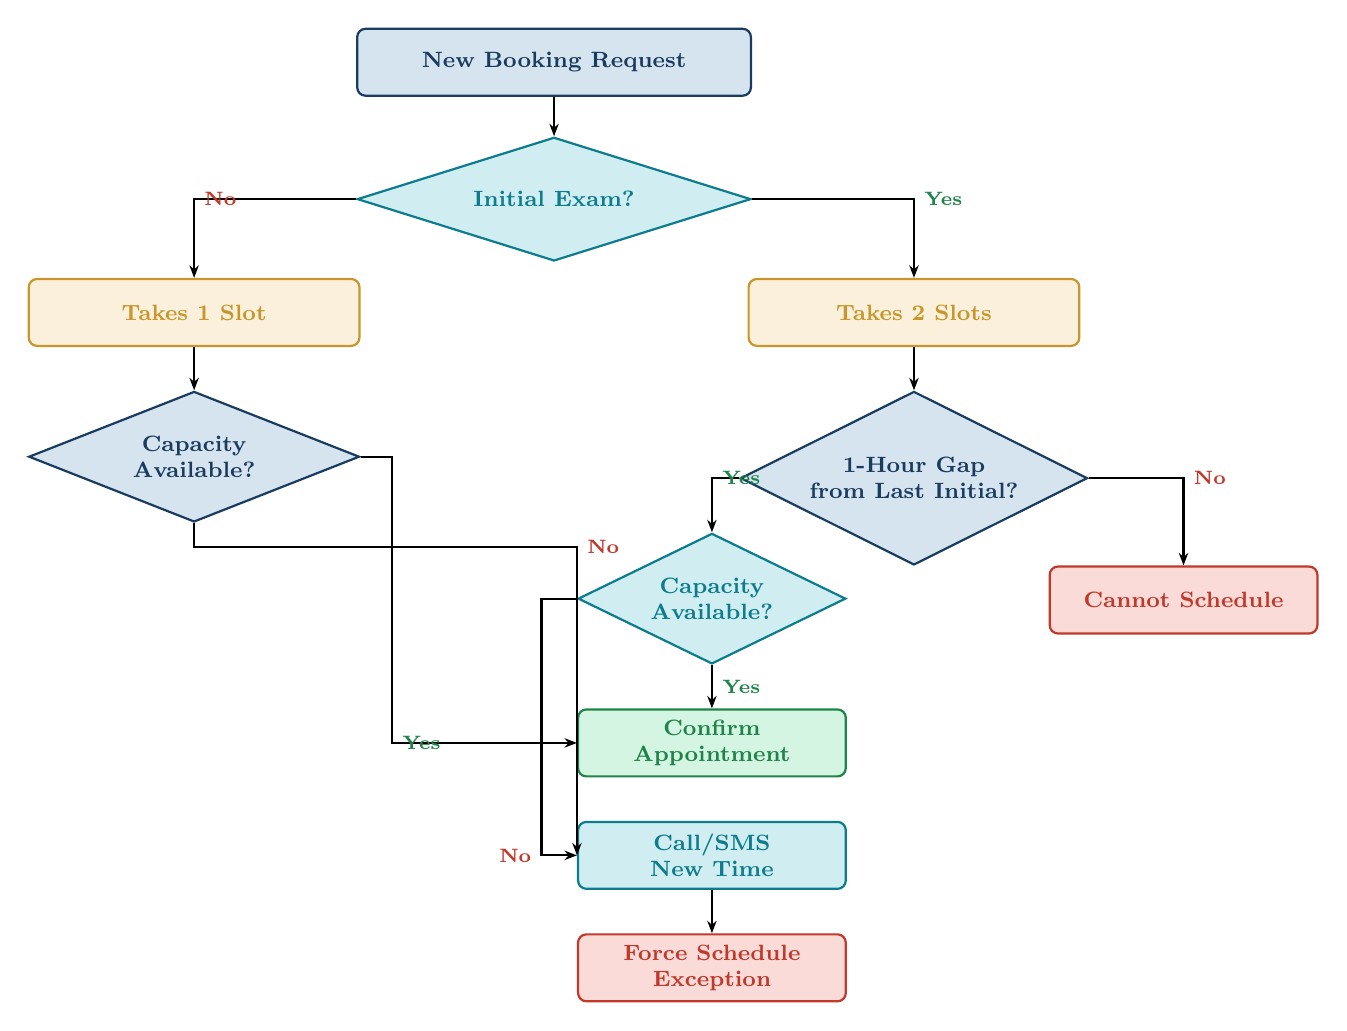
\begin{tikzpicture}[node distance=0.55cm,every node/.style={align=center}]
  \node[nB,minimum width=5cm]                  (req)  {New Booking Request};
  \node[dT,minimum width=5cm,below=0.5cm of req]       (init) {Initial Exam?};

  % --- Initial path (right branch) ---
  \node[nG,minimum width=4.2cm,below right=0.6cm and 1.2cm of init] (s2)   {Takes 2 Slots};
  \node[dB,minimum width=4.2cm,below=0.55cm of s2]                   (gap)  {1-Hour Gap \\ from Last Initial?};
  \node[nR,minimum width=3.4cm,below right=0.55cm and 0.6cm of gap]  (deny) {Cannot Schedule};
  \node[dT,minimum width=3.4cm,below left=0.55cm  and 0.6cm of gap]  (cap2) {Capacity \\ Available?};
  \node[nV,minimum width=3.4cm,below=0.55cm of cap2]                  (ok)   {Confirm \\ Appointment};
  \node[nT,minimum width=3.4cm,below=0.55cm of ok]                    (alt)  {Call/SMS \\ New Time};
  \node[nR,minimum width=3.4cm,below=0.55cm of alt]                   (force){Force Schedule \\ Exception};

  % --- Follow-up path (left branch) ---
  \node[nG,minimum width=4.2cm,below left=0.6cm and 1.2cm of init]  (s1)   {Takes 1 Slot};
  \node[dB,minimum width=4.2cm,below=0.55cm of s1]                   (cap1) {Capacity \\ Available?};

  \draw[arr](req)--(init);
  \draw[arr](init.east) -| node[LY]{Yes} (s2.north);
  \draw[arr](init.west) -| node[LN]{No}  (s1.north);
  \draw[arr](s2)--(gap);
  \draw[arr](gap.east) -| node[LN]{No}  (deny.north);
  \draw[arr](gap.west) -| node[LY]{Yes} (cap2.north);
  \draw[arr](cap2.south)-- node[LY,right]{Yes} (ok.north);
  \draw[arr](cap2.west)--++(-0.45,0)|- node[LN,left]{No} (alt.west);
  \draw[arr](s1)--(cap1);
  % cap1 yes -> ok  (horizontal connector)
  \draw[arr](cap1.east) -- ++(0.4,0) |- node[LY,right]{Yes} (ok.west);
  % cap1 no -> alt
  \draw[arr](cap1.south) -- ++(0,-0.3) -| node[LN,right]{No} (alt.west);
  \draw[arr](alt)--(force);
\end{tikzpicture}
\end{center}

%------------------------------------------------------------
\subsection{Back Office --- Outbound \& Cash Flow Operations}
%------------------------------------------------------------

The Back Office is the cash-flow engine, executing five critical daily workflows that protect attendance,
authorization compliance, and future booking continuity.

\begin{center}
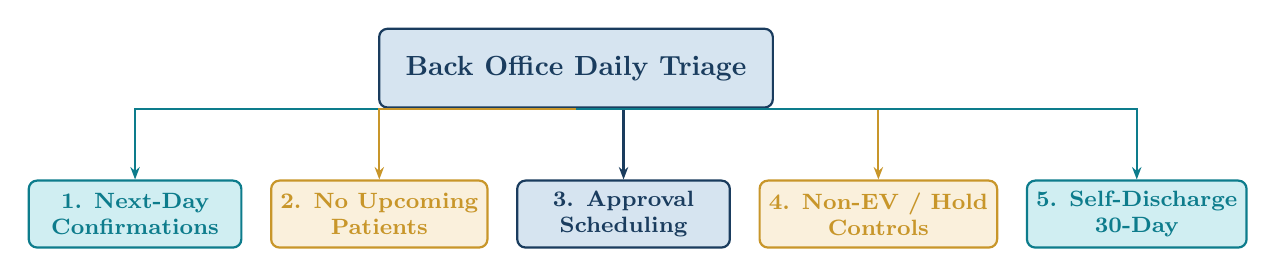
\begin{tikzpicture}[node distance=0.5cm and 0.45cm]
  \node[nB,minimum width=5cm,minimum height=1cm,font=\bfseries\normalsize] (triage)
    {Back Office Daily Triage};
  \node[nT,minimum width=2.7cm,below=0.9cm of triage,xshift=-5.6cm] (c1){1. Next-Day \\ Confirmations};
  \node[nG,minimum width=2.7cm,right=0.35cm of c1]                  (c2){2. No Upcoming \\ Patients};
  \node[nB,minimum width=2.7cm,right=0.35cm of c2]                  (c3){3. Approval \\ Scheduling};
  \node[nG,minimum width=2.7cm,right=0.35cm of c3]                  (c4){4. Non-EV / Hold \\ Controls};
  \node[nT,minimum width=2.7cm,right=0.35cm of c4]                  (c5){5. Self-Discharge \\ 30-Day};
  \draw[arr,AccentTeal]  (triage.south)-|(c1.north);
  \draw[arr,AccentGold]  (triage.south)-|(c2.north);
  \draw[arr,PrimaryBlue] (triage.south)-|(c3.north);
  \draw[arr,AccentGold]  (triage.south)-|(c4.north);
  \draw[arr,AccentTeal]  (triage.south)-|(c5.north);
\end{tikzpicture}
\end{center}

\subsubsection{Workflow 1: Next-Day Confirmations}

\begin{tcolorbox}[infobox,title={Confirmation Cycle --- Step by Step}]
\begin{enumerate}
  \item \textbf{Mass SMS Blast:} Send campaign via SimpleTexting to all next-day patients using the C/R/X instruction format.
  \item \textbf{2-Hour Hold:} Wait two hours before filtering and actioning responses.
  \item \textbf{Action Responses:}
    \begin{itemize}
      \item \textcolor{SuccessGreen}{\bfseries C / Confirm:} Mark as confirmed on schedule.
      \item \textcolor{WarningAmber}{\bfseries R (Reschedule):} Cancel current; book new appointment immediately.
      \item \textcolor{DangerRed}{\bfseries X (Cancel):} Document reason. If patient has future appointments $\rightarrow$ keep. If no future appointments $\rightarrow$ attempt to schedule; document failure reason if unsuccessful.
    \end{itemize}
  \item \textbf{Outbound Calls:} Call all non-respondents directly.
  \item \textbf{Audit Trail:} Every opened SMS thread must be actioned, logged, or assigned for follow-up before leaving the queue.
\end{enumerate}
\end{tcolorbox}

\begin{tcolorbox}[warnbox,title={SimpleTexting Search Rule}]
Do not search only for the single letter \textbf{``C''}. Patients may reply with \textbf{``Confirm''},
\textbf{``confirmed''}, or other natural-language responses. The agent must review opened threads and not rely only on exact-letter filtering.
\end{tcolorbox}

\vspace{0.4em}
\begin{tcolorbox}[statbox]
\begin{center}
  \large\bfseries Key Statistical Reality\\[0.5em]
  \begin{tabular}{ccc}
    \begin{tabular}{c}
      {\LARGE\bfseries\color{SuccessGreen}62\%}\\[2pt]
      {\small\color{MidGray}of non-respondents}\\
      {\small\color{MidGray}\emph{still show up}}
    \end{tabular}
    & \qquad &
    \begin{tabular}{c}
      {\LARGE\bfseries\color{DangerRed}20\%}\\[2pt]
      {\small\color{MidGray}of confirmed patients}\\
      {\small\color{MidGray}\emph{still No-Show}}
    \end{tabular}
  \end{tabular}\\[0.4em]
  \small\color{MidGray}\textit{Confirmation $\neq$ Attendance. \quad Non-response $\neq$ Cancellation.}
\end{center}
\end{tcolorbox}

\vspace{0.4em}
\begin{center}
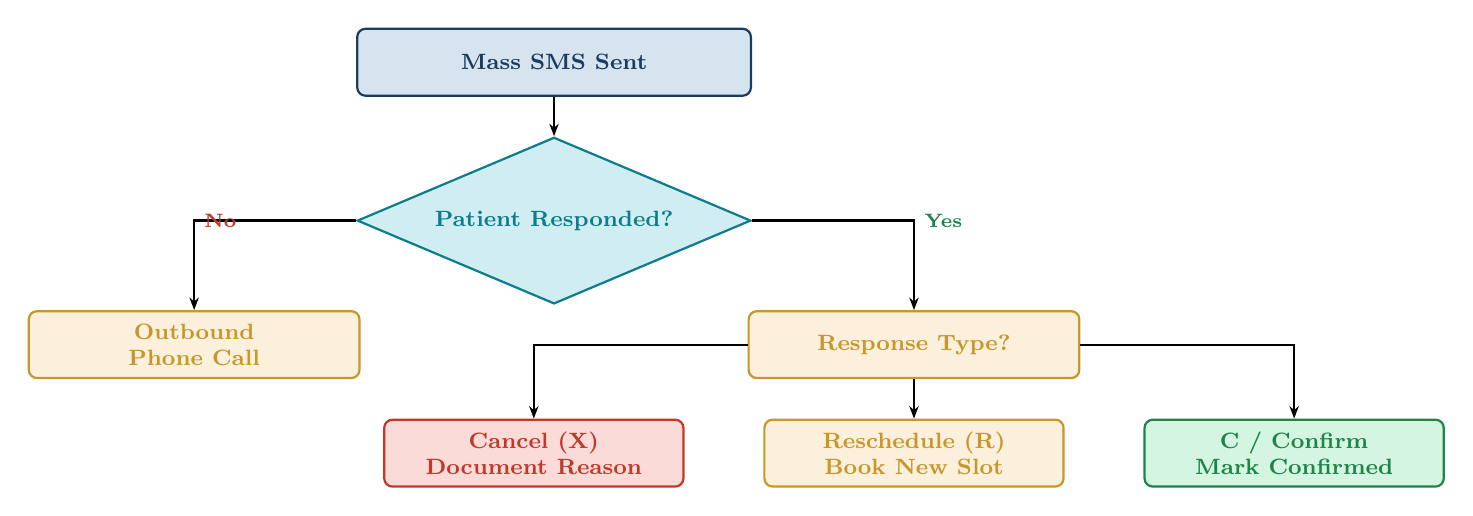
\begin{tikzpicture}[node distance=0.55cm,every node/.style={align=center}]
  \node[nB,minimum width=5cm]                     (sms)  {Mass SMS Sent};
  \node[dT,minimum width=5cm,below=0.5cm of sms]  (resp) {Patient Responded?};

  \node[nG,minimum width=4.2cm,below right=0.6cm and 1.2cm of resp] (type) {Response Type?};
  \node[nV,minimum width=3.8cm,below right=0.5cm and 0.8cm of type] (C) {C / Confirm \\ Mark Confirmed};
  \node[nG,minimum width=3.8cm,below=0.5cm of type]                  (R) {Reschedule (R) \\ Book New Slot};
  \node[nR,minimum width=3.8cm,below left=0.5cm  and 0.8cm of type] (X) {Cancel (X) \\ Document Reason};
  \node[nG,minimum width=4.2cm,below left=0.6cm  and 1.2cm of resp] (call){Outbound \\ Phone Call};

  \draw[arr](sms)--(resp);
  \draw[arr](resp.east) -| node[LY]{Yes} (type.north);
  \draw[arr](resp.west) -| node[LN]{No}  (call.north);
  \draw[arr](type.east) -| (C.north);
  \draw[arr](type)--(R);
  \draw[arr](type.west) -| (X.north);
\end{tikzpicture}
\end{center}

\subsubsection{Workflow 2: No Upcoming Appointments}

Agents pull a daily list of patients who attended a session yesterday but left without booking their next appointment. They proactively call \emph{and} SMS these patients to re-engage them before the gap widens.

\begin{tcolorbox}[rulebox,title={No Upcoming Control Rule}]
This workflow protects retention and visit continuity. A patient who leaves the clinic without a future appointment is a revenue-risk patient, even if they attended yesterday.
\end{tcolorbox}

\begin{center}
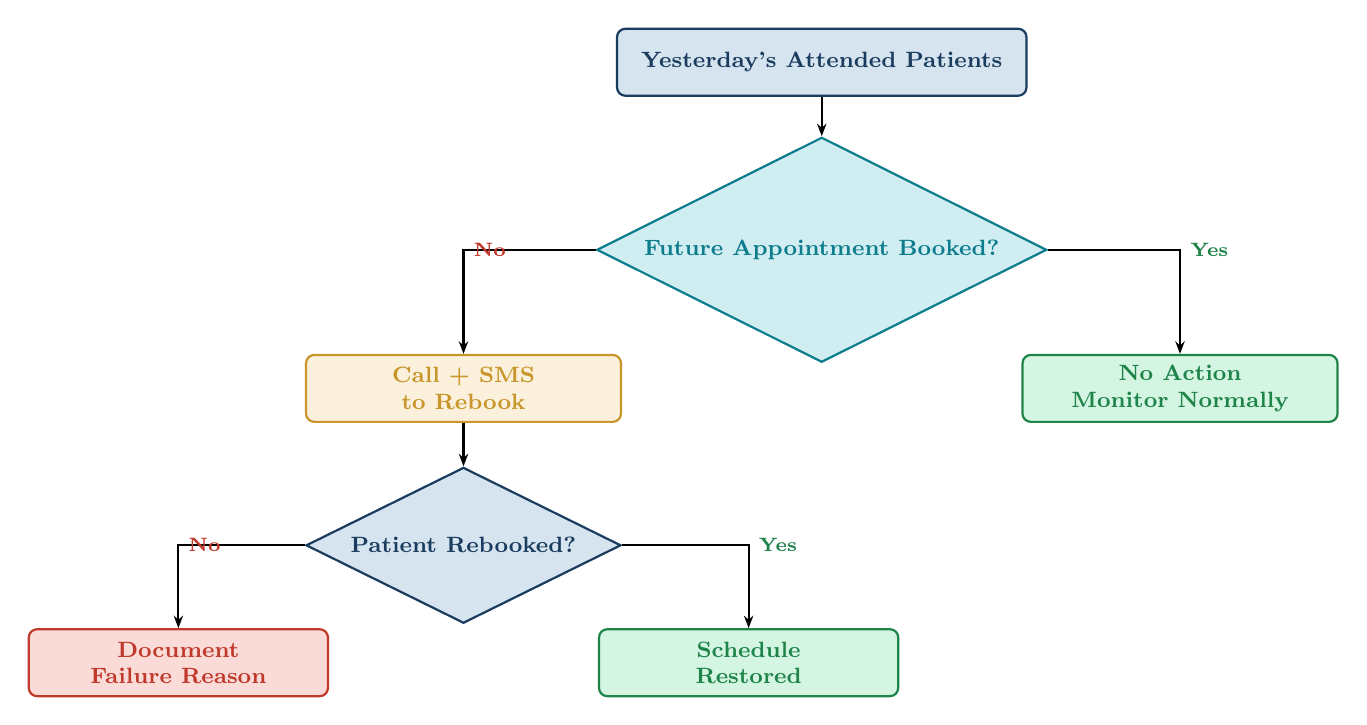
\begin{tikzpicture}[node distance=0.55cm,every node/.style={align=center}]
  \node[nB,minimum width=5.2cm] (list) {Yesterday's Attended Patients};
  \node[dT,minimum width=5.2cm,below=0.5cm of list] (future) {Future Appointment Booked?};
  \node[nV,minimum width=4.0cm,below right=0.6cm and 1.1cm of future] (done) {No Action \\ Monitor Normally};
  \node[nG,minimum width=4.0cm,below left=0.6cm and 1.1cm of future] (outreach) {Call + SMS \\ to Rebook};
  \node[dB,minimum width=4.0cm,below=0.55cm of outreach] (booked) {Patient Rebooked?};
  \node[nV,minimum width=3.8cm,below right=0.55cm and 0.7cm of booked] (saved) {Schedule \\ Restored};
  \node[nR,minimum width=3.8cm,below left=0.55cm and 0.7cm of booked] (reason) {Document \\ Failure Reason};

  \draw[arr](list)--(future);
  \draw[arr](future.east)-| node[LY]{Yes} (done.north);
  \draw[arr](future.west)-| node[LN]{No} (outreach.north);
  \draw[arr](outreach)--(booked);
  \draw[arr](booked.east)-| node[LY]{Yes} (saved.north);
  \draw[arr](booked.west)-| node[LN]{No} (reason.north);
\end{tikzpicture}
\end{center}

\subsubsection{Workflow 3: Insurance Approval Scheduling}

Approval updates represent immediate scheduling opportunities. Agents review yesterday's approvals daily; on Mondays, they review the full weekend backlog.

\begin{tcolorbox}[successbox,title={Approval Scheduling SOP}]
\begin{enumerate}
  \item Pull all new authorization approvals from the Authorization Team update.
  \item Confirm visit count, authorization window, expiration date, and case association.
  \item Call the patient immediately to schedule approved visits.
  \item If the patient does not answer, send SMS and document the outreach attempt.
  \item Avoid booking beyond the approved authorization window.
\end{enumerate}
\end{tcolorbox}

\subsubsection{Workflow 4: Non-EV and Hold Patient Controls}

\begin{tcolorbox}[warnbox,title={Insurance Status Management Rules}]
\begin{tabularx}{\linewidth}{L{3.0cm} X L{3.2cm}}
  \rowcolor{TableHead}
  \color{white}\textbf{Status} & \color{white}\textbf{Description} & \color{white}\textbf{Action} \\
  \textbf{Approval}
    & New authorized visits granted (Mon: review full weekend)
    & Call immediately to schedule \\
  \rowcolor{TableAlt}
  \textbf{Non-EV}
    & Visits exhausted; awaiting turnaround (e.g., 4-day cycle)
    & \textcolor{WarningAmber}{\bfseries Reschedule PAST turnaround date} \\
  \textbf{On Hold}
    & Missing referral, COB issue, or insurance change
    & \textcolor{DangerRed}{\bfseries Cancel ALL upcoming appts} \\
\end{tabularx}
\end{tcolorbox}

\begin{tcolorbox}[dangerbox,title={Critical Rule --- Hold Patients}]
Agents \textbf{MUST cancel all upcoming appointments} for On Hold patients. Failure = clinic treats patient for free = unbillable visit = direct revenue loss.
\end{tcolorbox}

\begin{tcolorbox}[warnbox,title={Non-EV Rule}]
Agents \textbf{MUST NOT cancel} Non-EV patients. Reschedule to a date \emph{after} the expected insurance turnaround window.
\end{tcolorbox}

\vspace{0.4em}
\begin{center}
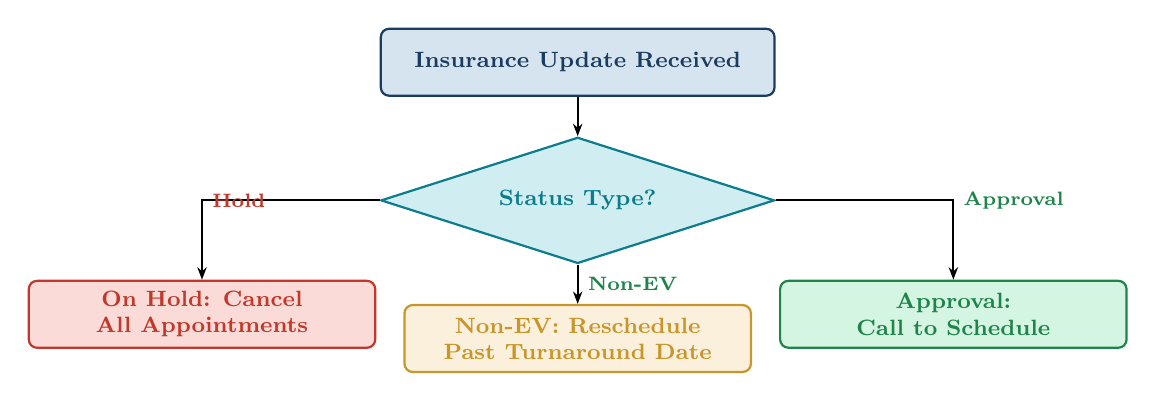
\begin{tikzpicture}[node distance=0.55cm,every node/.style={align=center}]
  \node[nB,minimum width=5cm]                    (ins)  {Insurance Update Received};
  \node[dT,minimum width=5cm,below=0.5cm of ins] (type) {Status Type?};
  \node[nV,minimum width=4.4cm,below right=0.6cm and 1.3cm of type] (appr){Approval: \\ Call to Schedule};
  \node[nG,minimum width=4.4cm,below=0.5cm of type]                  (nev) {Non-EV: Reschedule \\ Past Turnaround Date};
  \node[nR,minimum width=4.4cm,below left=0.6cm  and 1.3cm of type] (hold){On Hold: Cancel \\ All Appointments};

  \draw[arr](ins)--(type);
  \draw[arr](type.east) -| node[LY]{\scriptsize Approval} (appr.north);
  \draw[arr](type.south)-- node[LY,right]{\scriptsize Non-EV} (nev.north);
  \draw[arr](type.west) -| node[LN]{\scriptsize Hold} (hold.north);
\end{tikzpicture}
\end{center}

\subsubsection{Workflow 5: Self-Discharge --- Lost Patients (30-Day)}

Patients not attending for \textbf{30 days} are flagged as \emph{Self-Discharged}. Agents call to uncover the reason.

\begin{tcolorbox}[infobox,title={Self-Discharge Reasons \& Actions}]
\begin{tabularx}{\linewidth}{L{4.4cm} X}
  \rowcolor{TableHead}
  \color{white}\textbf{Reason} & \color{white}\textbf{Required Action} \\
  Medical issue / recovering    & Partial or full discharge \\
  \rowcolor{TableAlt}
  Relocated                     & Full discharge --- close chart \\
  Unhappy with clinic / PT      & Full discharge --- document feedback \\
  \rowcolor{TableAlt}
  Finished specific body part   & Partial discharge --- close case only; may return as New Case \\
  Fully recovered               & Full discharge \\
  \rowcolor{TableAlt}
  Wants to return               & Schedule new appointment immediately \\
\end{tabularx}
\end{tcolorbox}

\vspace{0.4em}
\begin{center}
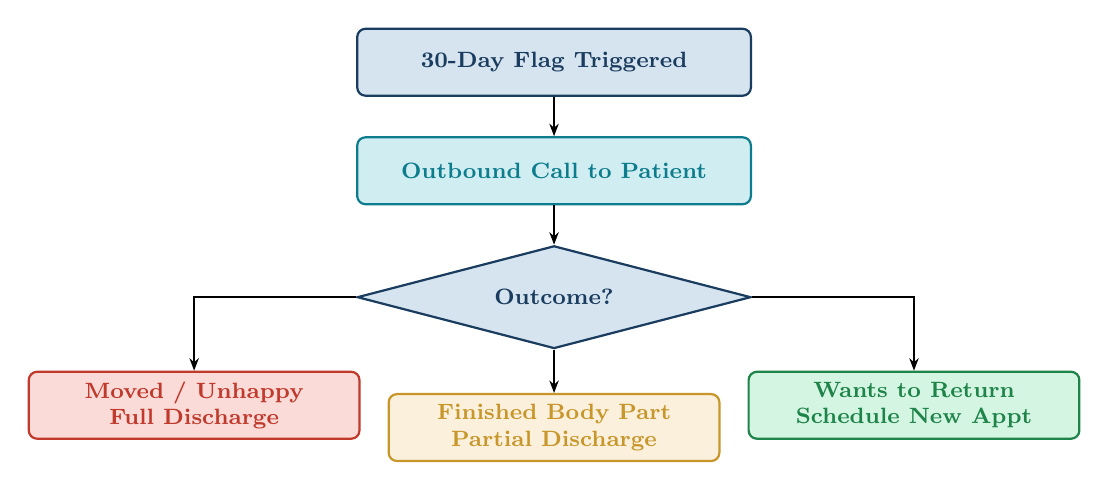
\begin{tikzpicture}[node distance=0.55cm,every node/.style={align=center}]
  \node[nB,minimum width=5cm]                    (flag) {30-Day Flag Triggered};
  \node[nT,minimum width=5cm,below=0.5cm of flag](call) {Outbound Call to Patient};
  \node[dB,minimum width=5cm,below=0.5cm of call](out)  {Outcome?};
  \node[nV,minimum width=4.2cm,below right=0.6cm and 1.2cm of out] (ret) {Wants to Return \\ Schedule New Appt};
  \node[nG,minimum width=4.2cm,below=0.55cm of out]                (part){Finished Body Part \\ Partial Discharge};
  \node[nR,minimum width=4.2cm,below left=0.6cm  and 1.2cm of out] (full){Moved / Unhappy \\ Full Discharge};

  \draw[arr](flag)--(call);
  \draw[arr](call)--(out);
  \draw[arr](out.east) -| (ret.north);
  \draw[arr](out.south)--(part.north);
  \draw[arr](out.west) -| (full.north);
\end{tikzpicture}
\end{center}

%------------------------------------------------------------
\subsection{Virtual Front Desk (VFD)}
%------------------------------------------------------------

The VFD operates as a remote receptionist for \textbf{17 clinics} that lack physical front desk staff.

\begin{tcolorbox}[infobox,title={VFD Operational Responsibilities}]
\begin{itemize}
  \item \textbf{Check-In:} Patient uses iPad/Kiosk (Name + DOB) $\rightarrow$ email triggers VFD agent $\rightarrow$ manual check-in in WebPT.
  \item \textbf{Check-Out (Intentionally Manual):} Self check-out is disabled by design. Agents enforce:
    \begin{enumerate}
      \item \textbf{Copay Collection:} Activate POS machine.
      \item \textbf{Future Booking:} Verify or book next appointment.
      \item \textbf{Visit Limit Warning:} Alert patient on last authorised visit; place on brief hold.
    \end{enumerate}
  \item \textbf{Re-Examination:} Every \textbf{10th visit} must be scheduled as a \emph{Re-examination} (shown \textcolor{DangerRed}{\textbf{red}} in WebPT), not a standard follow-up.
\end{itemize}
\end{tcolorbox}

\begin{tcolorbox}[dangerbox,title={VFD Legal and Billing Control}]
If a patient is checked in but not checked out, WebPT can show the patient as still present in the clinic.
This delays billing, disrupts operational reporting, and creates legal exposure regarding the patient's recorded whereabouts.
\end{tcolorbox}

\vspace{0.4em}
\begin{center}
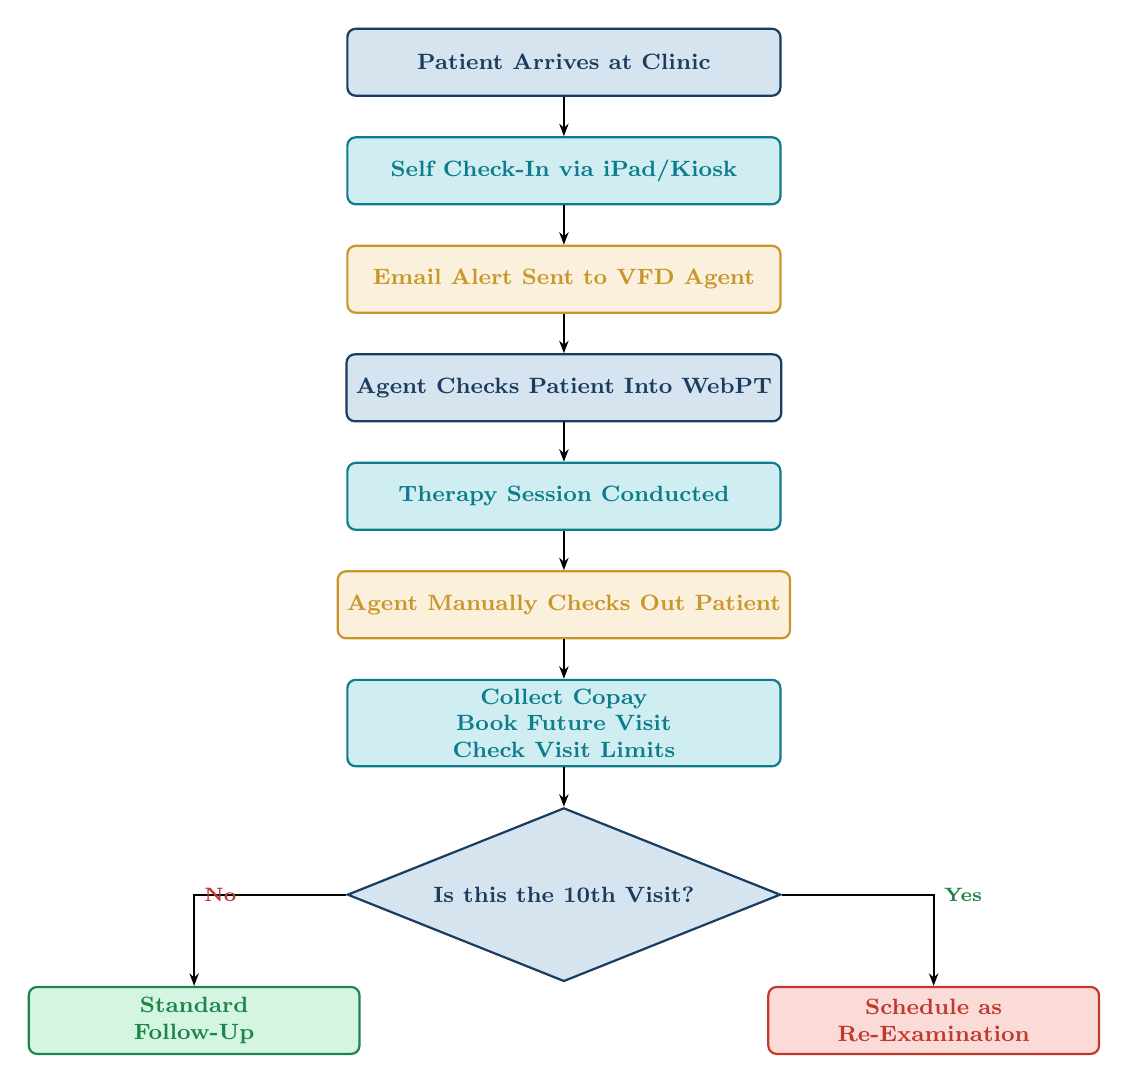
\begin{tikzpicture}[node distance=0.55cm,every node/.style={align=center}]
  \node[nB,minimum width=5.5cm]                      (arrive) {Patient Arrives at Clinic};
  \node[nT,minimum width=5.5cm,below=0.5cm of arrive](kiosk)  {Self Check-In via iPad/Kiosk};
  \node[nG,minimum width=5.5cm,below=0.5cm of kiosk] (email)  {Email Alert Sent to VFD Agent};
  \node[nB,minimum width=5.5cm,below=0.5cm of email] (checkin){Agent Checks Patient Into WebPT};
  \node[nT,minimum width=5.5cm,below=0.5cm of checkin](sess)   {Therapy Session Conducted};
  \node[nG,minimum width=5.5cm,below=0.5cm of sess]  (chkout) {Agent Manually Checks Out Patient};
  \node[nT,minimum width=5.5cm,below=0.5cm of chkout](controls){Collect Copay \\ Book Future Visit \\ Check Visit Limits};
  \node[dB,minimum width=5.5cm,below=0.5cm of controls](tenth)  {Is this the 10th Visit?};
  \node[nR,minimum width=4.2cm,below right=0.6cm and 1.2cm of tenth](re)  {Schedule as \\ Re-Examination};
  \node[nV,minimum width=4.2cm,below left=0.6cm  and 1.2cm of tenth](std) {Standard \\ Follow-Up};

  \draw[arr](arrive)--(kiosk);
  \draw[arr](kiosk)--(email);
  \draw[arr](email)--(checkin);
  \draw[arr](checkin)--(sess);
  \draw[arr](sess)--(chkout);
  \draw[arr](chkout)--(controls);
  \draw[arr](controls)--(tenth);
  \draw[arr](tenth.east) -| node[LY]{Yes} (re.north);
  \draw[arr](tenth.west) -| node[LN]{No}  (std.north);
\end{tikzpicture}
\end{center}

\newpage
%============================================================
\section{Daily Operating Control Dashboard}
%============================================================

This dashboard converts the workflows into management checkpoints for daily review,
staff supervision, and cash-flow forecasting.

\begin{tcolorbox}[infobox,title={Daily Control Points}]
\begin{tabularx}{\linewidth}{L{3.4cm} L{3.2cm} X L{3.1cm}}
  \rowcolor{TableHead}
  \color{white}\textbf{Control} & \color{white}\textbf{Owner} & \color{white}\textbf{Required Evidence} & \color{white}\textbf{Risk if Missed} \\
  Digital Queue Closure & Offline Desk & Queue cleared by 3:00 PM; unresolved conflicts documented & Schedule distortion \\
  \rowcolor{TableAlt}
  Next-Day Confirmations & Back Office & C/R/X responses processed; non-respondents called & No-Show leakage \\
  No Upcoming Review & Back Office & Yesterday's attended-without-future list called and SMSed & Retention loss \\
  \rowcolor{TableAlt}
  Authorization Updates & Back Office & New approvals scheduled; Non-EV rescheduled; Hold canceled & Unbillable visits \\
  VFD Check-Out & VFD & Copay, future visit, and visit-limit check completed & Billing/legal exposure \\
  \rowcolor{TableAlt}
  Case Selection Accuracy & Front Line / VFD & Correct active or new case selected in WebPT & Instant denial \\
\end{tabularx}
\end{tcolorbox}

\begin{center}
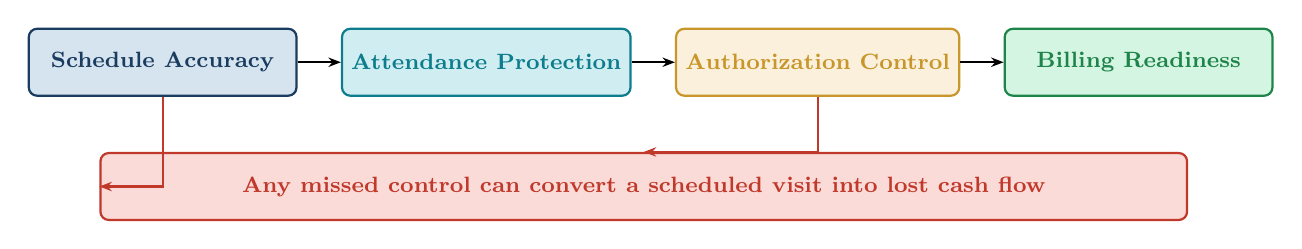
\begin{tikzpicture}[node distance=0.55cm and 0.55cm,every node/.style={align=center}]
  \node[nB,minimum width=3.4cm] (schedule) {Schedule Accuracy};
  \node[nT,minimum width=3.4cm,right=0.55cm of schedule] (attendance) {Attendance Protection};
  \node[nG,minimum width=3.4cm,right=0.55cm of attendance] (auth) {Authorization Control};
  \node[nV,minimum width=3.4cm,right=0.55cm of auth] (billing) {Billing Readiness};
  \draw[arr](schedule)--(attendance);
  \draw[arr](attendance)--(auth);
  \draw[arr](auth)--(billing);
  \node[nR,minimum width=13.8cm,below=0.7cm of attendance,xshift=2.0cm]
    (leak) {Any missed control can convert a scheduled visit into lost cash flow};
  \draw[arr,DangerRed](schedule.south)--++(0,-0.35)|-(leak.west);
  \draw[arr,DangerRed](auth.south)--++(0,-0.35)|-(leak.north);
\end{tikzpicture}
\end{center}

\newpage
%============================================================
\section{Systemic Errors \& Cash Flow Leakage Points}
%============================================================

Each of the following errors leads directly to denied claims, unbillable visits, or lost revenue.

\vspace{0.3em}

\begin{tcolorbox}[dangerbox,title={Error \#1 --- Multiple Cases Scheduling (Critical Billing Failure)}]
\textbf{What happens:} Patient returns for a new issue (e.g., Right Shoulder) but agent schedules under the old closed case (e.g., Left Knee) via the WebPT dropdown.\\[0.3em]
\textbf{System:} WebPT allows the booking without warning.\\[0.3em]
\textbf{Consequence:} Insurance claim \textbf{instantly denied} upon submission.
\end{tcolorbox}

\begin{tcolorbox}[dangerbox,title={Error \#2 --- Expired Authorization Scheduling}]
\textbf{What happens:} Agent books a date past the insurance authorization expiry.\\[0.3em]
\textbf{Example:} Booking May 27\textsuperscript{th} when authorization expired May 20\textsuperscript{th}.\\[0.3em]
\textbf{Consequence:} Visit is \textbf{completely unbillable} --- direct revenue loss.
\end{tcolorbox}

\begin{tcolorbox}[warnbox,title={Error \#3 --- Dummy Authorization Misinterpretation}]
\textbf{What happens:} Some insurers (e.g., Oxford Commercial) don't require formal auth. Billing enters \textbf{``0''} as placeholder. Agent misreads ``0'' as zero visits and cancels the patient.\\[0.3em]
\textbf{Consequence:} Revenue lost and patient relationship damaged unnecessarily.
\end{tcolorbox}

\begin{tcolorbox}[warnbox,title={Error \#4 --- SMS Leakage \& Response Processing Failures}]
\begin{itemize}
  \item Agent opens a message in SimpleTexting but fails to log or follow up.
  \item Searching for \textbf{``C''} misses patients who typed the full word \textbf{``Confirm''}.
\end{itemize}
\textbf{Consequence:} No-Show rates increase; confirmed slots remain at financial risk.
\end{tcolorbox}

\begin{tcolorbox}[dangerbox,title={Error \#5 --- Check-In / Check-Out Negligence (Legal Risk)}]
\textbf{What happens:} VFD agent checks in but forgets to check out.\\[0.3em]
\textbf{System appearance:} Patient appears in clinic \textbf{overnight}.\\[0.3em]
\textbf{Consequences:}
\begin{itemize}
  \item Billing delays and claim submission failures.
  \item \textbf{Severe legal liability} regarding unaccounted patient whereabouts.
\end{itemize}
\end{tcolorbox}

\begin{tcolorbox}[warnbox,title={Error \#6 --- Missing Medical Notes (Billing Halt)}]
\textbf{What happens:} PT forgets to close/sign daily note in WebPT.\\[0.3em]
\textbf{Consequence:} Billing cannot mark claim as \textbf{``Ready for Submission''} --- full cash flow halt for that visit.
\end{tcolorbox}

\begin{tcolorbox}[dangerbox,title={Error \#7 --- Inaccurate Eligibility Communication}]
\textbf{What happens:} Patient deemed ineligible but agent fails to cancel upcoming appointment.\\[0.3em]
\textbf{Consequence:} Clinic treats patient for free --- \textbf{fully unbillable visit}.
\end{tcolorbox}

\vspace{0.5em}
\begin{tcolorbox}[infobox,title={Error Risk Summary Matrix}]
\begin{tabularx}{\linewidth}{L{3.5cm} C{1.9cm} L{3.6cm} X}
  \rowcolor{TableHead}
  \color{white}\textbf{Error} & \color{white}\textbf{Severity} & \color{white}\textbf{Preventive Control} & \color{white}\textbf{Primary Impact} \\
  Multiple Cases Error           & \cellcolor{DangerRed!80}\color{white}Critical & Verify active/new case before booking & Instant claim denial \\
  \rowcolor{TableAlt}
  Expired Authorization          & \cellcolor{DangerRed!80}\color{white}Critical & Check authorization window and expiry date & Unbillable visit \\
  Dummy Auth Misread             & \cellcolor{WarningAmber!80}\color{white}High    & Confirm payer rule before cancellation & Lost revenue + patient churn \\
  \rowcolor{TableAlt}
  SMS Leakage                    & \cellcolor{WarningAmber!80}\color{white}High    & Review opened threads and natural replies & Increased No-Show rate \\
  Check-In/Out Negligence        & \cellcolor{DangerRed!80}\color{white}Critical & Manual check-out completion audit & Legal liability + billing delay \\
  \rowcolor{TableAlt}
  Missing Medical Notes          & \cellcolor{WarningAmber!80}\color{white}High    & PT note closure escalation & Cash flow halt \\
  Eligibility Communication Gap  & \cellcolor{DangerRed!80}\color{white}Critical & Cancel ineligible appointments immediately & Unbillable visit \\
\end{tabularx}
\end{tcolorbox}

\newpage
%============================================================
\section{Full Patient Lifecycle --- End-to-End Overview}
%============================================================

\vspace{0.3em}
\begin{center}
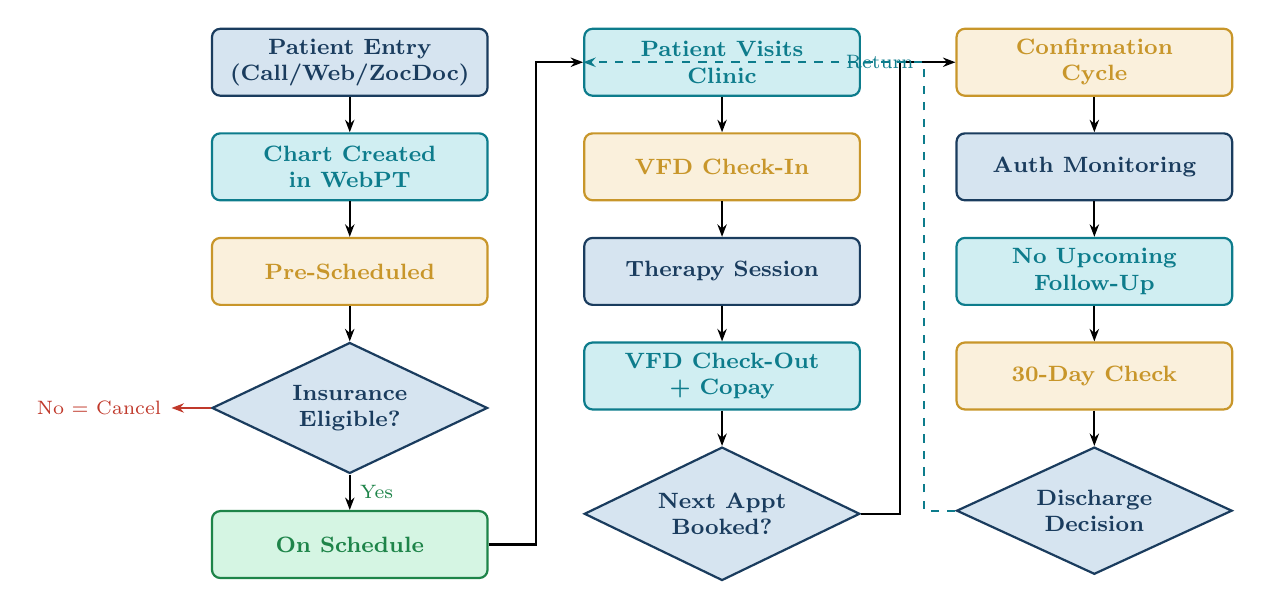
\begin{tikzpicture}[node distance=0.5cm and 1.2cm,
  every node/.style={align=center,font=\footnotesize\bfseries}]

  %------ COL 1: ENTRY ------
  \node[nB,minimum width=3.5cm] (entry)   {Patient Entry \\ (Call/Web/ZocDoc)};
  \node[nT,minimum width=3.5cm,below=0.45cm of entry]  (chart)   {Chart Created \\ in WebPT};
  \node[nG,minimum width=3.5cm,below=0.45cm of chart]  (presched){Pre-Scheduled};
  \node[dB,minimum width=3.5cm,below=0.45cm of presched](elig)   {Insurance \\ Eligible?};
  \node[nV,minimum width=3.5cm,below=0.45cm of elig]   (sched)   {On Schedule};

  %------ COL 2: VISIT CYCLE ------
  \node[nT,minimum width=3.5cm,right=1.2cm of entry]   (visit)   {Patient Visits \\ Clinic};
  \node[nG,minimum width=3.5cm,below=0.45cm of visit]  (checkin) {VFD Check-In};
  \node[nB,minimum width=3.5cm,below=0.45cm of checkin](sess)    {Therapy Session};
  \node[nT,minimum width=3.5cm,below=0.45cm of sess]   (chkout)  {VFD Check-Out \\ + Copay};
  \node[dB,minimum width=3.5cm,below=0.45cm of chkout] (nxtappt) {Next Appt \\ Booked?};

  %------ COL 3: MANAGEMENT ------
  \node[nG,minimum width=3.5cm,right=1.2cm of visit]   (conf)    {Confirmation \\ Cycle};
  \node[nB,minimum width=3.5cm,below=0.45cm of conf]   (authmon) {Auth Monitoring};
  \node[nT,minimum width=3.5cm,below=0.45cm of authmon](noup)    {No Upcoming \\ Follow-Up};
  \node[nG,minimum width=3.5cm,below=0.45cm of noup]   (thirty)  {30-Day Check};
  \node[dB,minimum width=3.5cm,below=0.45cm of thirty] (dc)      {Discharge \\ Decision};

  % COL1 arrows
  \draw[arr](entry)--(chart);
  \draw[arr](chart)--(presched);
  \draw[arr](presched)--(elig);
  \draw[arr](elig)--node[right,font=\scriptsize\color{SuccessGreen}]{Yes}(sched);
  \draw[arr](sched.east)--++(0.6,0)|-(visit.west);

  % COL2 arrows
  \draw[arr](visit)--(checkin);
  \draw[arr](checkin)--(sess);
  \draw[arr](sess)--(chkout);
  \draw[arr](chkout)--(nxtappt);
  \draw[arr](nxtappt.east)--++(0.5,0)|-(conf.west);

  % COL3 arrows
  \draw[arr](conf)--(authmon);
  \draw[arr](authmon)--(noup);
  \draw[arr](noup)--(thirty);
  \draw[arr](thirty)--(dc);

  % Feedback loop
  \draw[arr,dashed,AccentTeal,thick]
    (dc.west)--++(-0.4,0)|-node[left,font=\scriptsize]{Return}(visit.west);

  % Eligibility NO branch
  \draw[arr,DangerRed](elig.west)--++(-0.5,0)
    node[left,font=\scriptsize\color{DangerRed}]{No = Cancel};
\end{tikzpicture}
\end{center}

%============================================================
% CLOSING
%============================================================
\vspace{1.0em}
\begin{tcolorbox}[enhanced,colback=PrimaryBlue,colframe=AccentGold,
    boxrule=2pt,arc=6pt,left=12pt,right=12pt,top=10pt,bottom=10pt]
  \begin{center}
    \color{white}\large\bfseries Core Objective\\[0.5em]
    \color{SoftBlue}\normalsize
    Patient acquisition, retention, schedule optimisation, and cash flow preservation\\
    through rigorous compliance with billing and authorisation protocols.\\[0.5em]
    \color{AccentGold}\small\textit{Every scheduling decision, confirmation action,
    and discharge classification has a direct financial consequence.}
  \end{center}
\end{tcolorbox}

\vspace{0.6em}
\begin{center}
  \color{MidGray}\small
  \textit{AI Department --- Prepared by Eng.\ Abdulrahman Hamdi, AI Engineer --- 2026}
\end{center}

\end{document}